% siminos/CLE/Hilbert.tex
% $Author: siminos $ $Date: 2009-12-19 02:59:14 +0100 (Sat, 19 Dec 2009) $

%\subsection{\label{s:Hilbert}Hilbert basis approach}

The most common approach to symmetry reduction is through the
use of a Hilbert basis of invariant polynomials. One computes
a (non-unique) basis of linearly independent polynomials,
invariant under the action of the symmetry group (\cf
\refref{gatermannHab,ChossLaut00} for a discussion of
methods) and either rewrites the dynamics in this basis or
maps the solutions to the polynomial variables.
The reader is referred to the book of Gilmore and
Lettelier\rf{GL-Gil07b} for a very detailed discussion of
symmetry reduction, through the use of invariant polynomials\ES{Also Chossat and Lauterbach?}.

It will be convenient to rewrite the system in real variables
$x=x_1+ i\, x_2\,,\ y=y_1+i\, x_2$ as
\beq
\begin{split}
	\dot{x}_1 &= -\sigma x_1 + \sigma y_1\cont
	\dot{x}_2 &= -\sigma x_2 + \sigma y_2\cont
	\dot{y}_1 &= (\RerCLor-z) x_1 - \ImrCLor x_2 -y_1-e y_2 \cont
	\dot{y}_2 &= \ImrCLor x_1 + (\RerCLor-z) x_2 + e y_1- y_2\cont
	\dot{z} \; &= -b z + x_1 y_1 + x_2 y_2\,.
	\label{eq:CLeR}
\end{split}
\eeq

The action \refeq{eq:SO2cle} of $\SOn{2}$ on $\Rls{5}$ is then given by
\beq
	X \mapsto  \Rot{\theta}X\,,
	\label{eq:SO2act}
\eeq
where
\beq
	\Rot{\theta}=	\left(\barr{ccccc}
				\cos(\theta) & -\sin(\theta) & 0	   & 0		    & 0\\
				\sin(\theta) & \cos(\theta)  & 0	   & 0		    & 0\\		
				0	     & 	0	     & \cos(\theta) & -\sin(\theta) & 0\\
				0	     &  0	     & \sin(\theta) & \cos(\theta) & 0\\
				0	     &  0	     & 0	    & 0		   & 1\\	
			\earr\right)\,,\ \ \theta\in[0,2\pi)\,,
    \label{eq:RotCLe5d}
\eeq
and $X=(x_1\,,\ x_2\,,\ y_1\,,\ y_2\,,\ z)$.

CLE take the form
\beq
\begin{split}
 \dot{x}_1 &= -\sigma x_1 + \sigma y_1\cont
 \dot{x}_2 &= -\sigma x_2 + \sigma y_2\cont
 \dot{y}_1 &= (\rho_1-z) x_1 -\rho_2 x_2 -y_1 -e y_2\cont
 \dot{y}_2 &= (\rho_1-z) x_2 +\rho_2 x_1 -y_2 +e y_1\cont
 \dot{z} &= x_1 y_1 + x_2 y_2 -b z\,.	
\end{split}
\eeq
Gilmore and Letellier\rf{GL-Gil07b} compute a Hilbert basis
for the action \refeq{eq:SO2act} of $\SOn{2}$ on \Rls{5}  
and use it for symmetry reduction of the Zeghlache-Mandel system\rf{ZeMa85}, 
conjugate to \cLe, with $e=-\ImrCLor$. For reasons explained in \refsect{s:introCLE}
we do not follow their choice of system but we can still utilize their invariant
basis that reads
\beq
\begin{split}
	u_1 &= x_1^2+x_2^2 \cont
	u_2 &= y_1^2+y_2^2 \cont
	u_3 &= x_1 y_2-x_2 y_1\cont
	u_4 &= x_1 y_1+x_2 y_2\cont
	u_5 &= z\,.
	\label{eq:ipLaser}
\end{split}
\eeq
As often is the case with Hilbert bases the $u_i$'s are linearly 
independent but functionally dependent through 
\beq
 	u_1u_2 -u_3^2-u_4^2 =0\,.
	\label{eq:syzLaser}
\eeq
Such a relation is called a syzygy and its presence corresponds to the fact
that symmetry reduction leads to state space dimension reduction by the
dimension of the group, here by one.

%%%%%%%%%%%%%%%%%%%%%%%%%%%%%%%%%%%%%%%%%%%%%%%%%%%%%%%%%%%%%%%%%%
\begin{figure}[ht]
\begin{center}
  (\textit{a})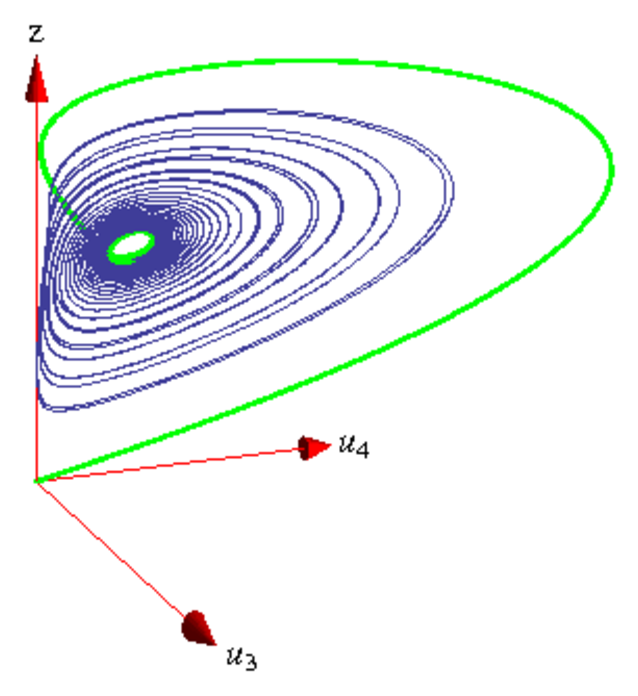
\includegraphics[width=0.35\textwidth]{../figs/CLEip1}
~~~~(\textit{b})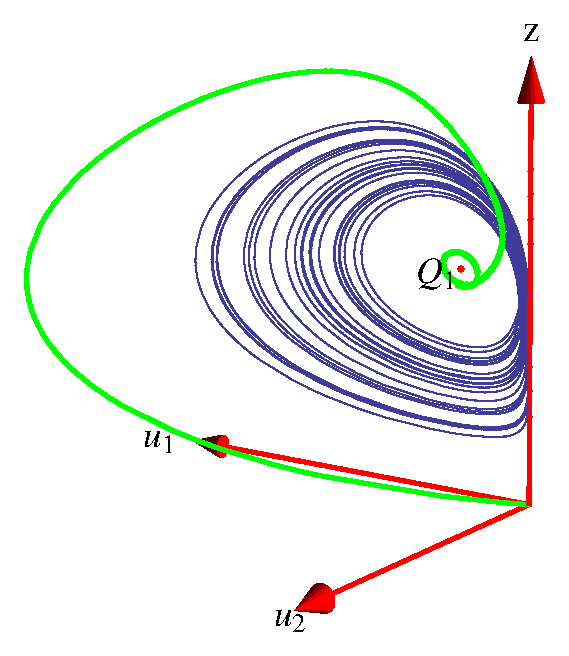
\includegraphics[width=0.36\textwidth]{../figs/CLEip2}
\end{center}
\caption[Orbit space projection of Complex Lorenz flow:
Invariant polynomials basis]{ \Statesp\ portraits of \cLe\
dynamics for $e=1/10$, $\ImrCLor=0$ in \reducedsp,
invariant polynomials basis \refeq{eq:ipLaser}.
    }
\label{fig:CLEip}
\end{figure}
%%%%%%%%%%%%%%%%%%%%%%%%%%%%%%%%%%%%%%%%%%%%%%%%%%%%%%%%%%%%%%%%


We use the chain rule with \refeq{eq:ipLaser} and \refeq{eq:CLeR}
\beq
 \dot{u}_i=\frac{\partial u_i}{\partial x_j}\dot{x}_j
 \,,
\ee{ChainRul}
and express the result in invariant polynomials:
    \ES{mathematica notebook:CLEtransfJac.nb
    {\bf PC:} Changed $z$ to $u_5$; have not checked the algebra}\
    \ES{Rechecked algebra by hand, keeping $\rho_2\neq 0$. $u_3$ and $u_4$ where permuted. I will have to check
		the figures for consistency.}
\beq
\begin{split}
  \dot{u}_1 &=2\,\sigma\,(u_4-u_1)\,,\\
  \dot{u}_2 &=-2\left(\,u_2 - \rho_2\, u_3 -\,(\rho_1-u_5)\,u_4\right)\,,\\
  \dot{u}_3 &=-(\sigma\, +1)\,u_3+\rho_2\, u_1+e\, u_4\,,\\
  \dot{u}_4 &=-(\sigma\, +1)\,u_4+\,(\rho_1-u_5)\,u_1+\sigma\, u_2-e\,u_3\,,\\
  \dot{u}_5 &=u_4-b\, u_5\,.
\end{split}
\label{eq:CLEip}
\eeq
For visualization purposes, rather than integrating
\refeq{eq:CLEip}, we map solutions of \refeq{eq:CLe} to the
$u_i$'s, \reffig{fig:CLEip}. In most projections the folding
mechanism is hidden from view since the dynamics is squeezed
near the $z$-axis, invariant polynomials being multiplicative
in equivariant variables.

Nevertheless we can now easily identify a suitable Poincar\'e
section as one that contains the $z$-axis and
the \reqv, here defined by the condition $u_1=u_4$\ES{explain}.
Eventhough in \cLe\ case we could use one of the $u_i$'s as
a coordinate to construct a return map, for more general flows
a dynamically intrisic parametrization is needed.
Following \refref{Christiansen97} we construct the first return map 
of \reffig{fig:CLEipRM} using as coordinate the
Euclidean length along the intersection of the unstable
manifold of \REQV{}{1} with the Poincar\'e surface of section,
measured from \REQV{}{1}, as described in \refsect{s:Poincare}.

Unfortunately the utility of Hilbert basis methods is restricted 
by the fact that determination of a Hilbert basis becomes computationally
prohibitive as the dimension of the system and/or group
increases\rf{gatermannHab,ChossLaut00}. Typical
computations are constrained to dimension smaller than ten. 
As our goal is to quotient continuous symmetries of
high-dimensional flows, specifically those arising from
truncations of the \KS\ and Navier-Stokes flows
and thus we need an efficient framework.



\subsection{\label{s:Poincare}Symmetry reduced return map}

Successive trajectory intersections with a {\em Poincar\'e
section}, a $(d-1)$-dim\-ens\-ion\-al hypersurface
\ES{use term hypersurface instead of submanifold also for 
slices?} 
or a set of
hypersurfaces $\PoincS$ embedded in the $d$-dim\-ens\-ion\-al
{\statesp} $\pS$, define the {\em Poincar\'e return map}
$\PoincM({\ssp})$, a $(d-1)$-dim\-ens\-ion\-al map of form
\index{map!return}
\index{Poincar\'e return map}
\PC{draw figure}
\index{first return function}
\beq
\ssp' = \PoincM({\ssp})
          =  \flow{\tau(\ssp)}{\ssp}
\,,\qquad
\ssp', \ssp \in \PoincS
\,.
\ee{PoincMap}
Here the {\em first return function} $\tau(\ssp)$--sometimes
referred to as the {\em ceiling function}--is the time of
flight to the next section for a trajectory starting at $\ssp$.
The choice of the section hypersurface $\PoincS$ is altogether
arbitrary. \ES{enter some criteria for our choice. Draw section
in invariant polynomial figures.}

We begin by sprinkling evenly points
$\{\ssp^{(1)},\ssp^{(2)},\cdots,\ssp^{(N-1)}\}$ between the
\reqv\ point $\ssp_{\REQV{}{1}}=\ssp^{(0)}$ and point  $\ssp=
\ssp^{(N)}$, along the $1d$ intersection of \Poincare\ section and
unstable manifold continuation $\ssp^{(k)} \in \hat{W}^u_{(1)}$ of the unstable ${\bf
\hat{e}}^{(1)}$ eigen\-plane (we shall omit the
eigen\-direction label ${}_{(1)}$ in what follows). Then the
arclength in Euclidean metric (for the luck of a more natural metric) 
from \reqv\ point $\ssp_{\REQV{}{1}}=\ssp^{(0)}$ to $\ssp=
\ssp^{(N)}$ is given by
% \beq
% s^2 = \lim_{N\to\infty}
%            \sum_{k=1}^N g_{ij} \, d\ssp^{(k)}_i d\ssp^{(k)}_j
% \,,\qquad
%         d\ssp^{(k)}_i = \ssp^{(k)}_i - \ssp^{(k-1)}_i
% \,.
% \ee{arcLength}
% For the lack of a better idea
% (perhaps the dynamically determined $g = \jMps^T\jMps$
% would be a more natural metric?)
% let us measure arclength in the Euclidian metric,
% $g_{ij} = \delta_{ij}$, so
\beq
s = \lim_{N\to\infty}
         \left(\sum_{k=1}^N \left(d\ssp^{(k)}\right)^2\right)^{1/2}
\,.
\ee{EuclArcl}
By definition $f^{\tau(\ssp)}(\ssp) \in \hat{W}^u_{(j)}$, so
$f^t(\ssp)$ induces a $1d$ map $s(s_0,\tau) =
s(f^{\tau(\xInit)}(\xInit))$.

%%%%%%%%%%%%%%%%%%%%%%%%%%%%%%%%%%%%%%%%%%%%%%%%%%%%%%%%%%%%%%%%%%
\begin{figure}[ht]
\begin{center}
%   (\textit{a})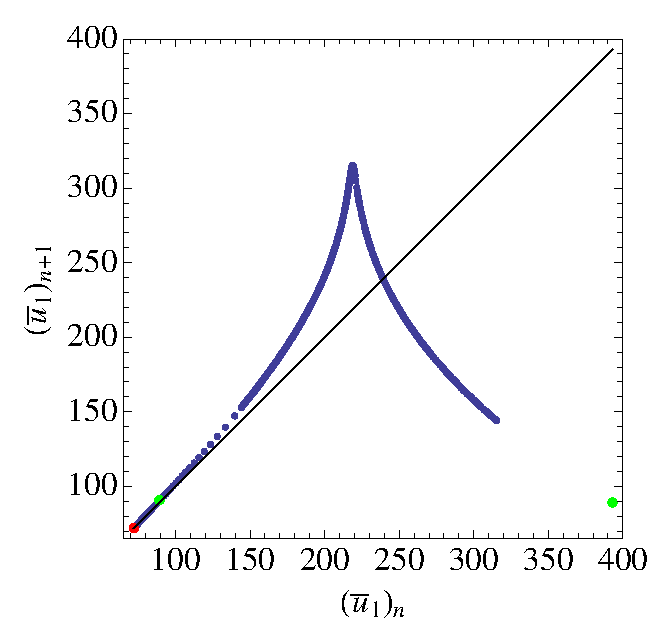
\includegraphics[width=0.35\textwidth]{../figs/CLEipRMu1}
%  ~~~~(\textit{b})
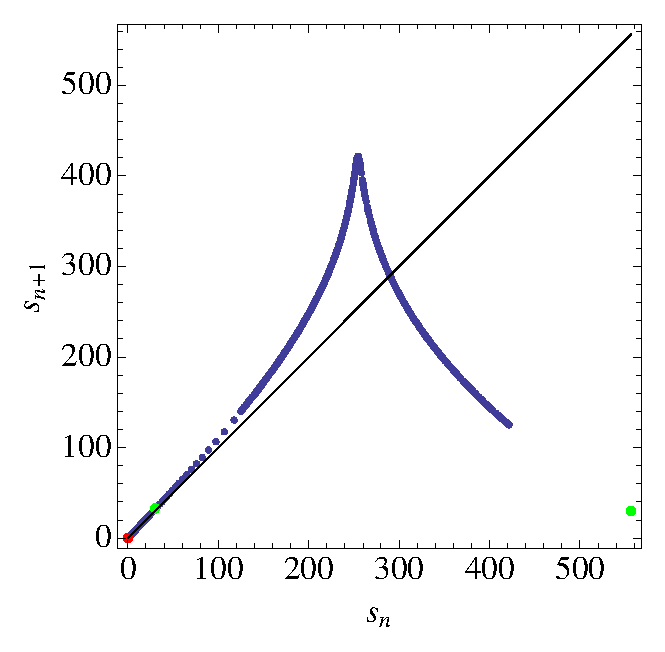
\includegraphics[width=0.35\textwidth]{../figs/CLEipRM}
\end{center}
\caption[Return map for Complex Lorenz flow, invariant polynomials]
{Return map to the \Poincare\
surface of section $u_1=u_4$ for \CLe\ with $e=1/10$, $\ImrCLor=0$,
projected on invariant polynomials \refeq{eq:ipLaser}.
% (a) The return map coordinate is $u_1$, (b)
The return map coordinate is the Euclidean
length along the \Poincare\ section of the unstable manifold of $E_1$.
    }
\label{fig:CLEipRM}
\end{figure}
%%%%%%%%%%%%%%%%%%%%%%%%%%%%%%%%%%%%%%%%%%%%%%%%%%%%%%%%%%%%%%%%

{\em \Turn s} are points on the unstable
manifold for which the local unstable manifold curvature diverges
for forward iterates of the map, \ie, points at which the manifold
folds back onto itself arbitrarily sharply.
For our purposes,
approximate \turn s suffice.
The $1d$ curve $\hat{W}^u_{(1)}$ starts out linear at
$\ssp_{\REQV{}{1}}$, then gently curves until it folds back sharply
at `\turn' along a possible heteroclinic connection to \EQV{0} 
and then nearly retraces itself. 

The trick is to figure out a good {\em base segment} to the
nearest {\turn} $L=[0,s_{b}]$, and after the foldback assign
to $s(\ssp,t)>s_{b}$ the nearest point $s$ on the base
segment. Since here the stable manifold contraction is strong, the
2nd coordinate connecting $s(\ssp,t) \to s$ can be neglected.

Armed with this intrinsic curvilinear coordinate
parametrization, we are now in a position to construct a
1-dimensional model of the dynamics on the \nws. If
$\hat{\ssp}_n$ is the $n$th Poincar\'e section of a
trajectory in neighborhood of $\ssp_\stagn$, and $s_n$ is the
corresponding curvilinear coordinate, then $s_{n+1} = f^{\tau_n}(s_n)$
models the full \statesp\ dynamics $\hat{\ssp}_n \to
\hat{\ssp}_{n+1}$. We approximate $f(s_n)$ by a smooth,
continuous 1-dimensional map $f : L_\stagn \to L_\stagn$ by taking
$\hat{\ssp}_n \in L_\stagn$, and assigning to
$\hat{\ssp}_{n+1}$ the nearest base segment point
$s_{n+1}=s(\hat{\ssp}_{n+1})$. The return map turns out to
be unimodal, binary symbolic dynamics are easilly constructed
and fixed points of the map up to length
$7$ systematically obtained. A multiple shooting rootine is then
used to determine the corresponding relative periodic orbits of
\cLe\ to machine precission.


